\documentclass{article}

\usepackage{csquotes}
\usepackage[margin=0.5in]{geometry}
\usepackage{graphicx}
\usepackage{rotating}
\usepackage[section]{placeins}

\title{FPGABoy Documentation}
\author{Luke Wren}

\begin{document}

\pagenumbering{gobble}
\maketitle
\tableofcontents
\newpage
\pagenumbering{arabic}

\section{What?}

FPGABoy is an open source portable games console, designed from scratch. It is also...
\begin{itemize}
\item An open source PCB layout
\item Designed with KiCAD open source PCB editor
\item An open source CPU, graphics and bus architecture
\item Based on the RISC-V open source instruction set
\item Synthesised and taped out with iCEStorm open source FPGA toolchain
\end{itemize}

\begin{displayquote}
\textit{If you say open source one more time I'm gonna nut instantly} - Oscar Wilde
\end{displayquote}

\subsection{Logic Design}

The heart of the design is a Lattice iCE40-HX8k FPGA, containing 7680 LUT4s and flipflops. The logic was designed from scratch, using synthesisable Verilog. This includes:
\begin{itemize}
\item RV32EC-compatible 32-bit CPU design
	\begin{itemize}
	\item E: embedded profile (reduced register set)
	\item C: compressed instruction extension, for higher code density
	\end{itemize}
\item Graphics pipeline
	\begin{itemize}
	\item Don't expect much, it's about as powerful as a Gameboy Advance
	\item Includes some MODE7-like functionality which allows drawing perspective-mapped textured planes, by providing per-scanline affine texture transformation. Think MarioKart
	\end{itemize}
\item AHB Lite 3.0-compatible multi-master busfabric
\item Other peripherals
	\begin{itemize}
	\item External SRAM controller
	\item Display controller
	\item DMA master
	\item Interrupt controller
	\item GPIO controller (buttons!)
	\item Serial port etc.
	\end{itemize}
\end{itemize}

Some attempt is made in this document to describe the operation of these hardware blocks, but if you are looking for nitty-gritty detail, the best documentation is the files ending with \texttt{.v}.

That a free synthesis tool can cram all this logic into one of the cheapest FPGAs on the market is tremendously impressive. Hopefully we will one day have a situation similar to software compilers, where free tools such as GCC are industry standards.

\subsection{PCB}

The board is a 4-layer stackup:

\begin{enumerate}
\item Signal + GND Fill
\item GND plane
\item Power planes
\item Signal + GND Fill
\end{enumerate}

It is intended to be suitable for low-cost PCB prototyping services such as iTead. Board dimensions are 50mm $\times$ 50mm, which fits into the cheapest size category on iTead. For the most part, it sticks to the following minimum specifications:

\begin{itemize}
\item Track width 0.15mm
\item Copper-copper clearance 0.15mm
\item Soldermask-copper clearance 0.1mm
\item Soldermask width 0.1mm
\item Via drill 0.3mm
\item Annular ring 0.15mm (i.e. via diameter 0.6mm)
\end{itemize}

The only exception is some 0.5mm vias underneath the BGA. Strictly this is out of specification for iTead, but they claim to have a 90 $\mu$m drill registration, so we'll see how it goes.

The iCE40-HX8k FPGA is packaged in a 256-pin 0.8mm BGA, which \textit{can be} reflowed by a hobbyist with a hot air gun or a frying pan (best to choose a HASL finish so that contacts are pretinned). The 132-pin 0.5mm BGA has sufficient IO for our needs, but iTead does not manufacture at the tolerance required for such a fine pitch.


\section{CPU Architecture}

\begin{sidewaysfigure}[!htb]
\caption{ReVive architectural block diagram}
\centering
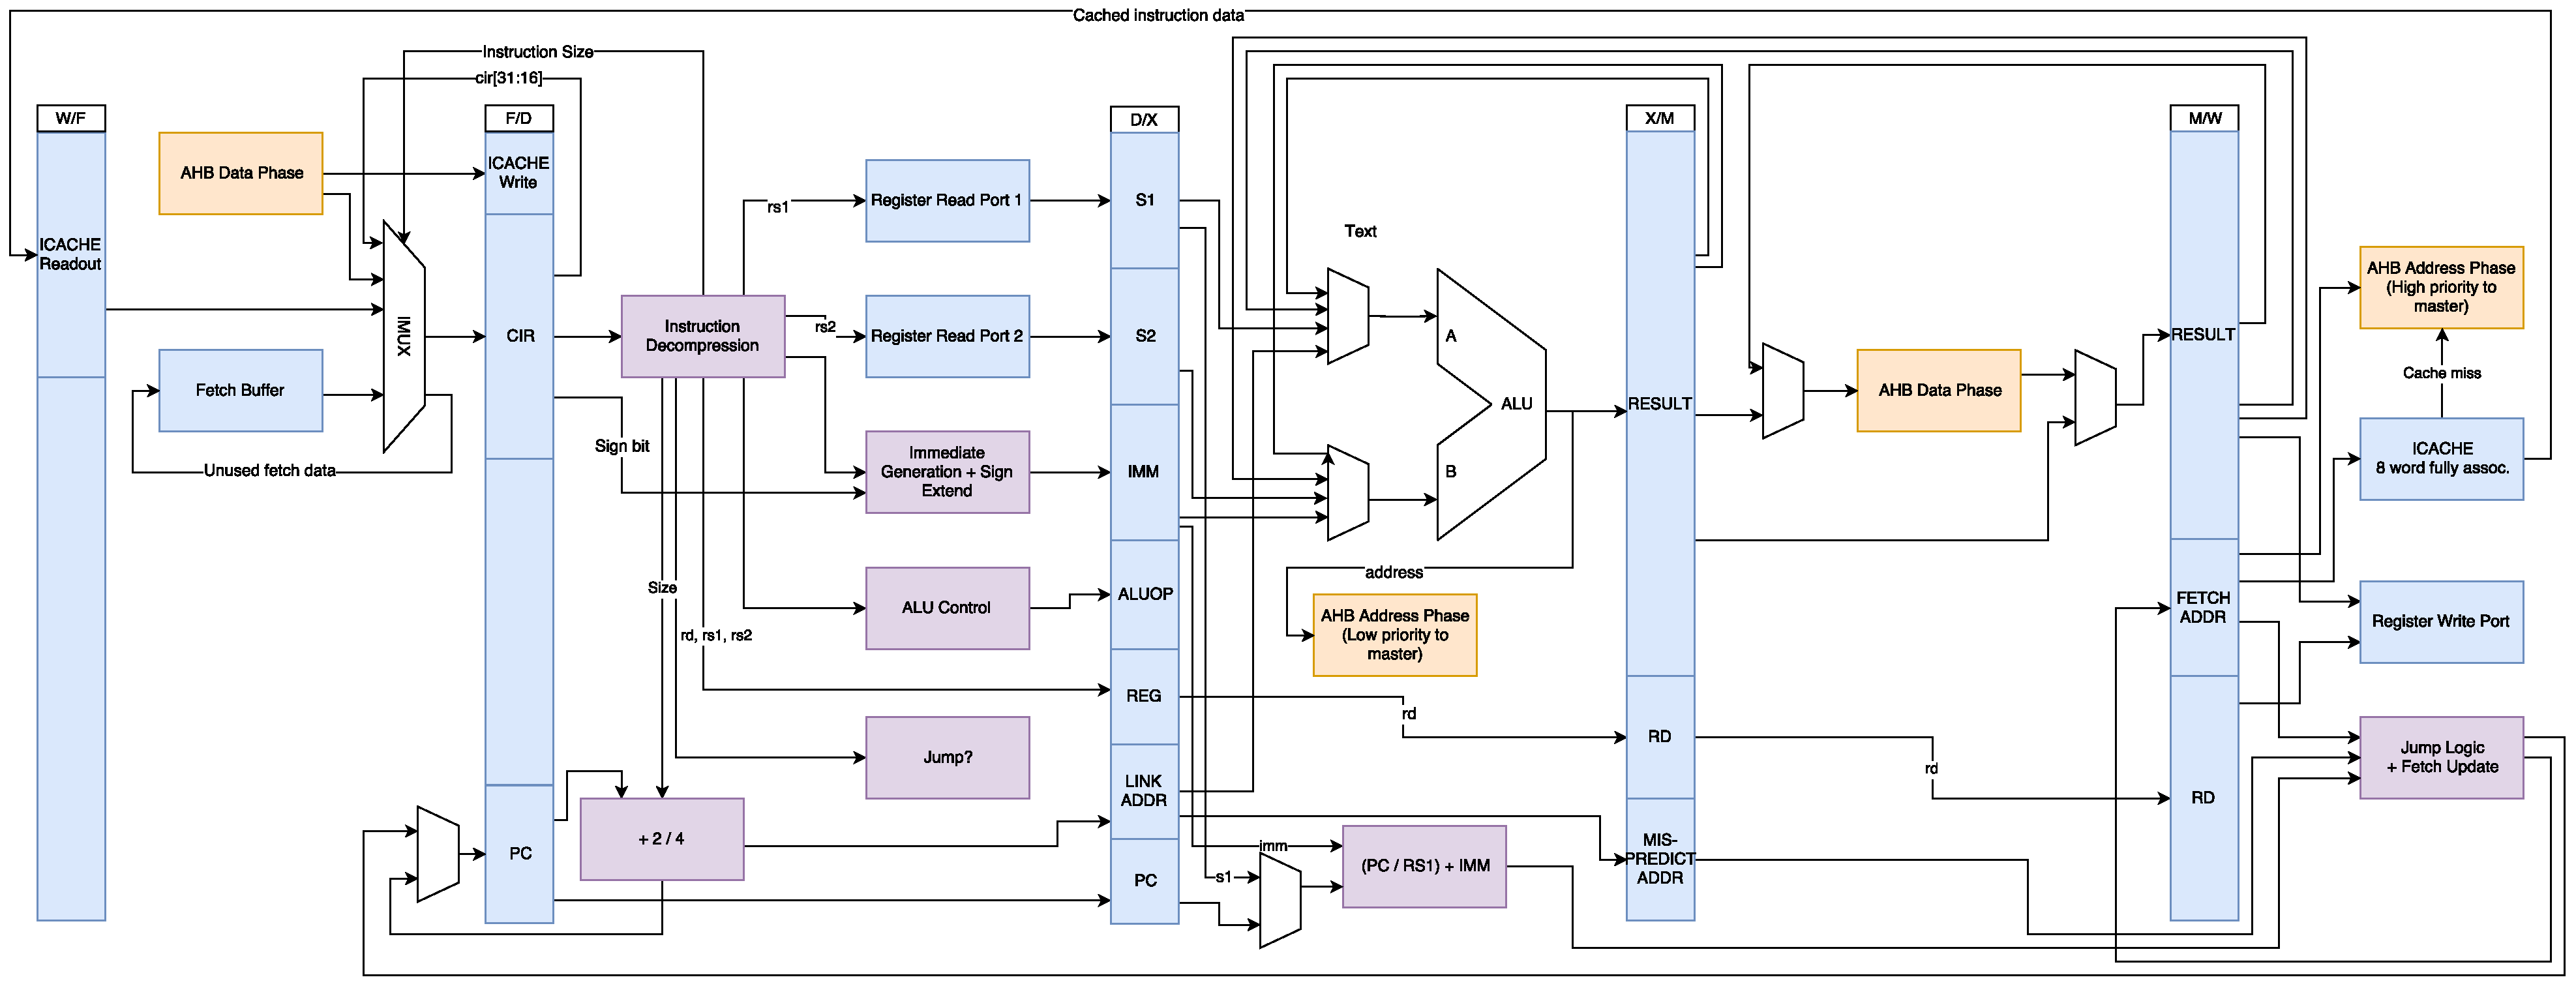
\includegraphics[width=0.9\textwidth]{diagrams/cpu_full.pdf}
\end{sidewaysfigure}

ReVive is a 32-bit processor based on the RISC V (hereafter RV) instruction set architecture. The name seemed appropriate for what is supposed to be a return to the glory days of games programming, when NULL pointers were just pointers to the start of ROM, and programmers were real programmers who wrote their \textit{own} polygon rasterisers, dammit.

The diagram shown here is a simplified block diagram of the core. Not shown is:
\begin{itemize}
\item The full and specific contents of the pipeline registers
\item The forwarding/bypass network which shortens data hazards to improve pipeline throughput
\item Additional hardware in ICACHE which helps to support unaligned code fetches
\item Interrupt entry/exit hardware
\item The ready/valid handshakes on pipe stages which allow them to NOP later stages, and stall prior ones
\item Hardware registers such as PC, and PC update logic
\item Pipeline flushing signals for branch mispredict
\end{itemize}

Overall this is a fairly standard RISC-style processor pipeline. The tall blue boxes represent the registers at the boundaries of two pipe stages. The nomenclature used in the diagram is:

\begin{itemize}
\item \texttt{F}: fetch
\item \texttt{D}: decode
\item \texttt{X}: execute
\item \texttt{M}: memory access (load/store)
\item \texttt{W}: register writeback
\end{itemize}

The processor has a single AHB-lite busmaster; the instruction fetcher and the load/store stage need to share it, and the instruction fetch takes priority.

Branches are speculated, according to the static prediction scheme described in the RV ISA manual:

\begin{itemize}
\item Backward branches are predicted to be taken, on the assumption that loops will run at least twice on average.
\item Forward branches are predicted not taken; the ISA manual advises that compilers should put more likely code on this path.
\end{itemize}

RISC-V compressed instructions achieve respectable code density, but it's no Thumb-2. The small instruction cache helps to tame the fetch bandwidth, so that load/stores and other system masters will still see some appreciable fraction of the bus bandwidth.

\subsection{Fetch Logic}

The \texttt{F} stage always provides \texttt{D} with 32 bits of fresh instruction data, in the canonical RISC-V order (halfword-wise little-endian). There are four sources for this data:

\begin{itemize}
\item AHB busmaster with access to system memory map
\item ICACHE. A small, fully-associative cache with random eviction
\item An \texttt{F}-local 16-bit buffer containing the unused second half of a previous word
\item The second halfword of the current instruction register of \texttt{D}, in the case that \texttt{D} found the last instruction to be 16-bit
\end{itemize}

\subsubsection {Sequential Code}
In sequential code, the ICACHE will be queried during \texttt{W}, as to whether it has the next aligned word. (We can guarantee the word will be aligned, as \texttt{F} buffers unused halfwords from prior accesses.)

The query response is combinatorial, and is used to decide whether to assert an AHB access during the address phase. Successful queries will result in cached read data appearing on the next clock edge, for use by \texttt{F}.

\texttt{F} is concurrent with the AHB data phase, except for a small muxing layer at the end which assembles the instruction word from AHB data, buffered data and cached data.

Following an unsuccessful ICACHE query, \texttt{F} will write the AHB data into the cache, evicting one word of its present contents. \textit{The same address must not appear more than once in the cache}, as the query logic is based on a non-priority sum of product encoder.

\subsubsection{Jumps}

Upon a jump or taken branch, \texttt{F}'s halfword buffer is invalidated, and the \texttt{CIR} is ignored.

Aligned jumps are otherwise no different from sequential code: the ICACHE is queried with the word access, and AHB supplies the data if ICACHE does not have it.

Unaligned jumps (i.e., halfword-aligned but not word-aligned) are more painful, as we may need to perform two accesses to fetch the required data.

The logic is as such:

\begin{enumerate}
\item \texttt{W} queries the cache with the address containing the first halfword and, in parallel, unconditionally fetches the second halfword via AHB
\item 
	\begin{itemize}
	\item After a cache hit, both required words will be available at the end of \texttt{F}. We have not lost any cycles.
	\item After a cache miss, \texttt{W} will stall stages \texttt{D,X,M}, and issue a second access over AHB, to fetch the first halfword			\end{itemize}
\item For fetched halfwords 0, 1, 2, 3:
	\begin{itemize}
	\item 0 is discarded
	\item 1, 2 are sent to \texttt{D}
	\item 3 is stored in \texttt{F}'s halfword buffer
	\end{itemize}
\end{enumerate} 

After this, we return to the sequential code steady-state.

\subsection{Jumps and Branches}

Due to the pipelined nature of AHB, we are unable to jump or to take branches in fewer than 2 cycles:

\begin{itemize}
\item Cycle 0: AHB address phase to fetch jump/branch instruction
\item Cycle 1: AHB data phase for fetch of jump/branch. Next instruction is in address phase concurrently.
\item Cycle 2: Jump/branch instruction is now available to \texttt{D}, and can be (quickly) used to control the new address phase.
\item The immediately following instruction is already in data phase
\end{itemize}

This gives the following cycle costs, assuming full speculation:
\begin{itemize}
\item Jump: 2 cycles
\item Predicted, non-taken branch: 1 cycle
\item Predicted, taken branch: 2 cycles (same as jump)
\item Branch mispredict: 4 cycles
\end{itemize}

The branch prediction scheme is static: take backward branches, and do not take forward branches.

\section{Graphics Pipeline}

\begin{figure}[!htb]
\centering
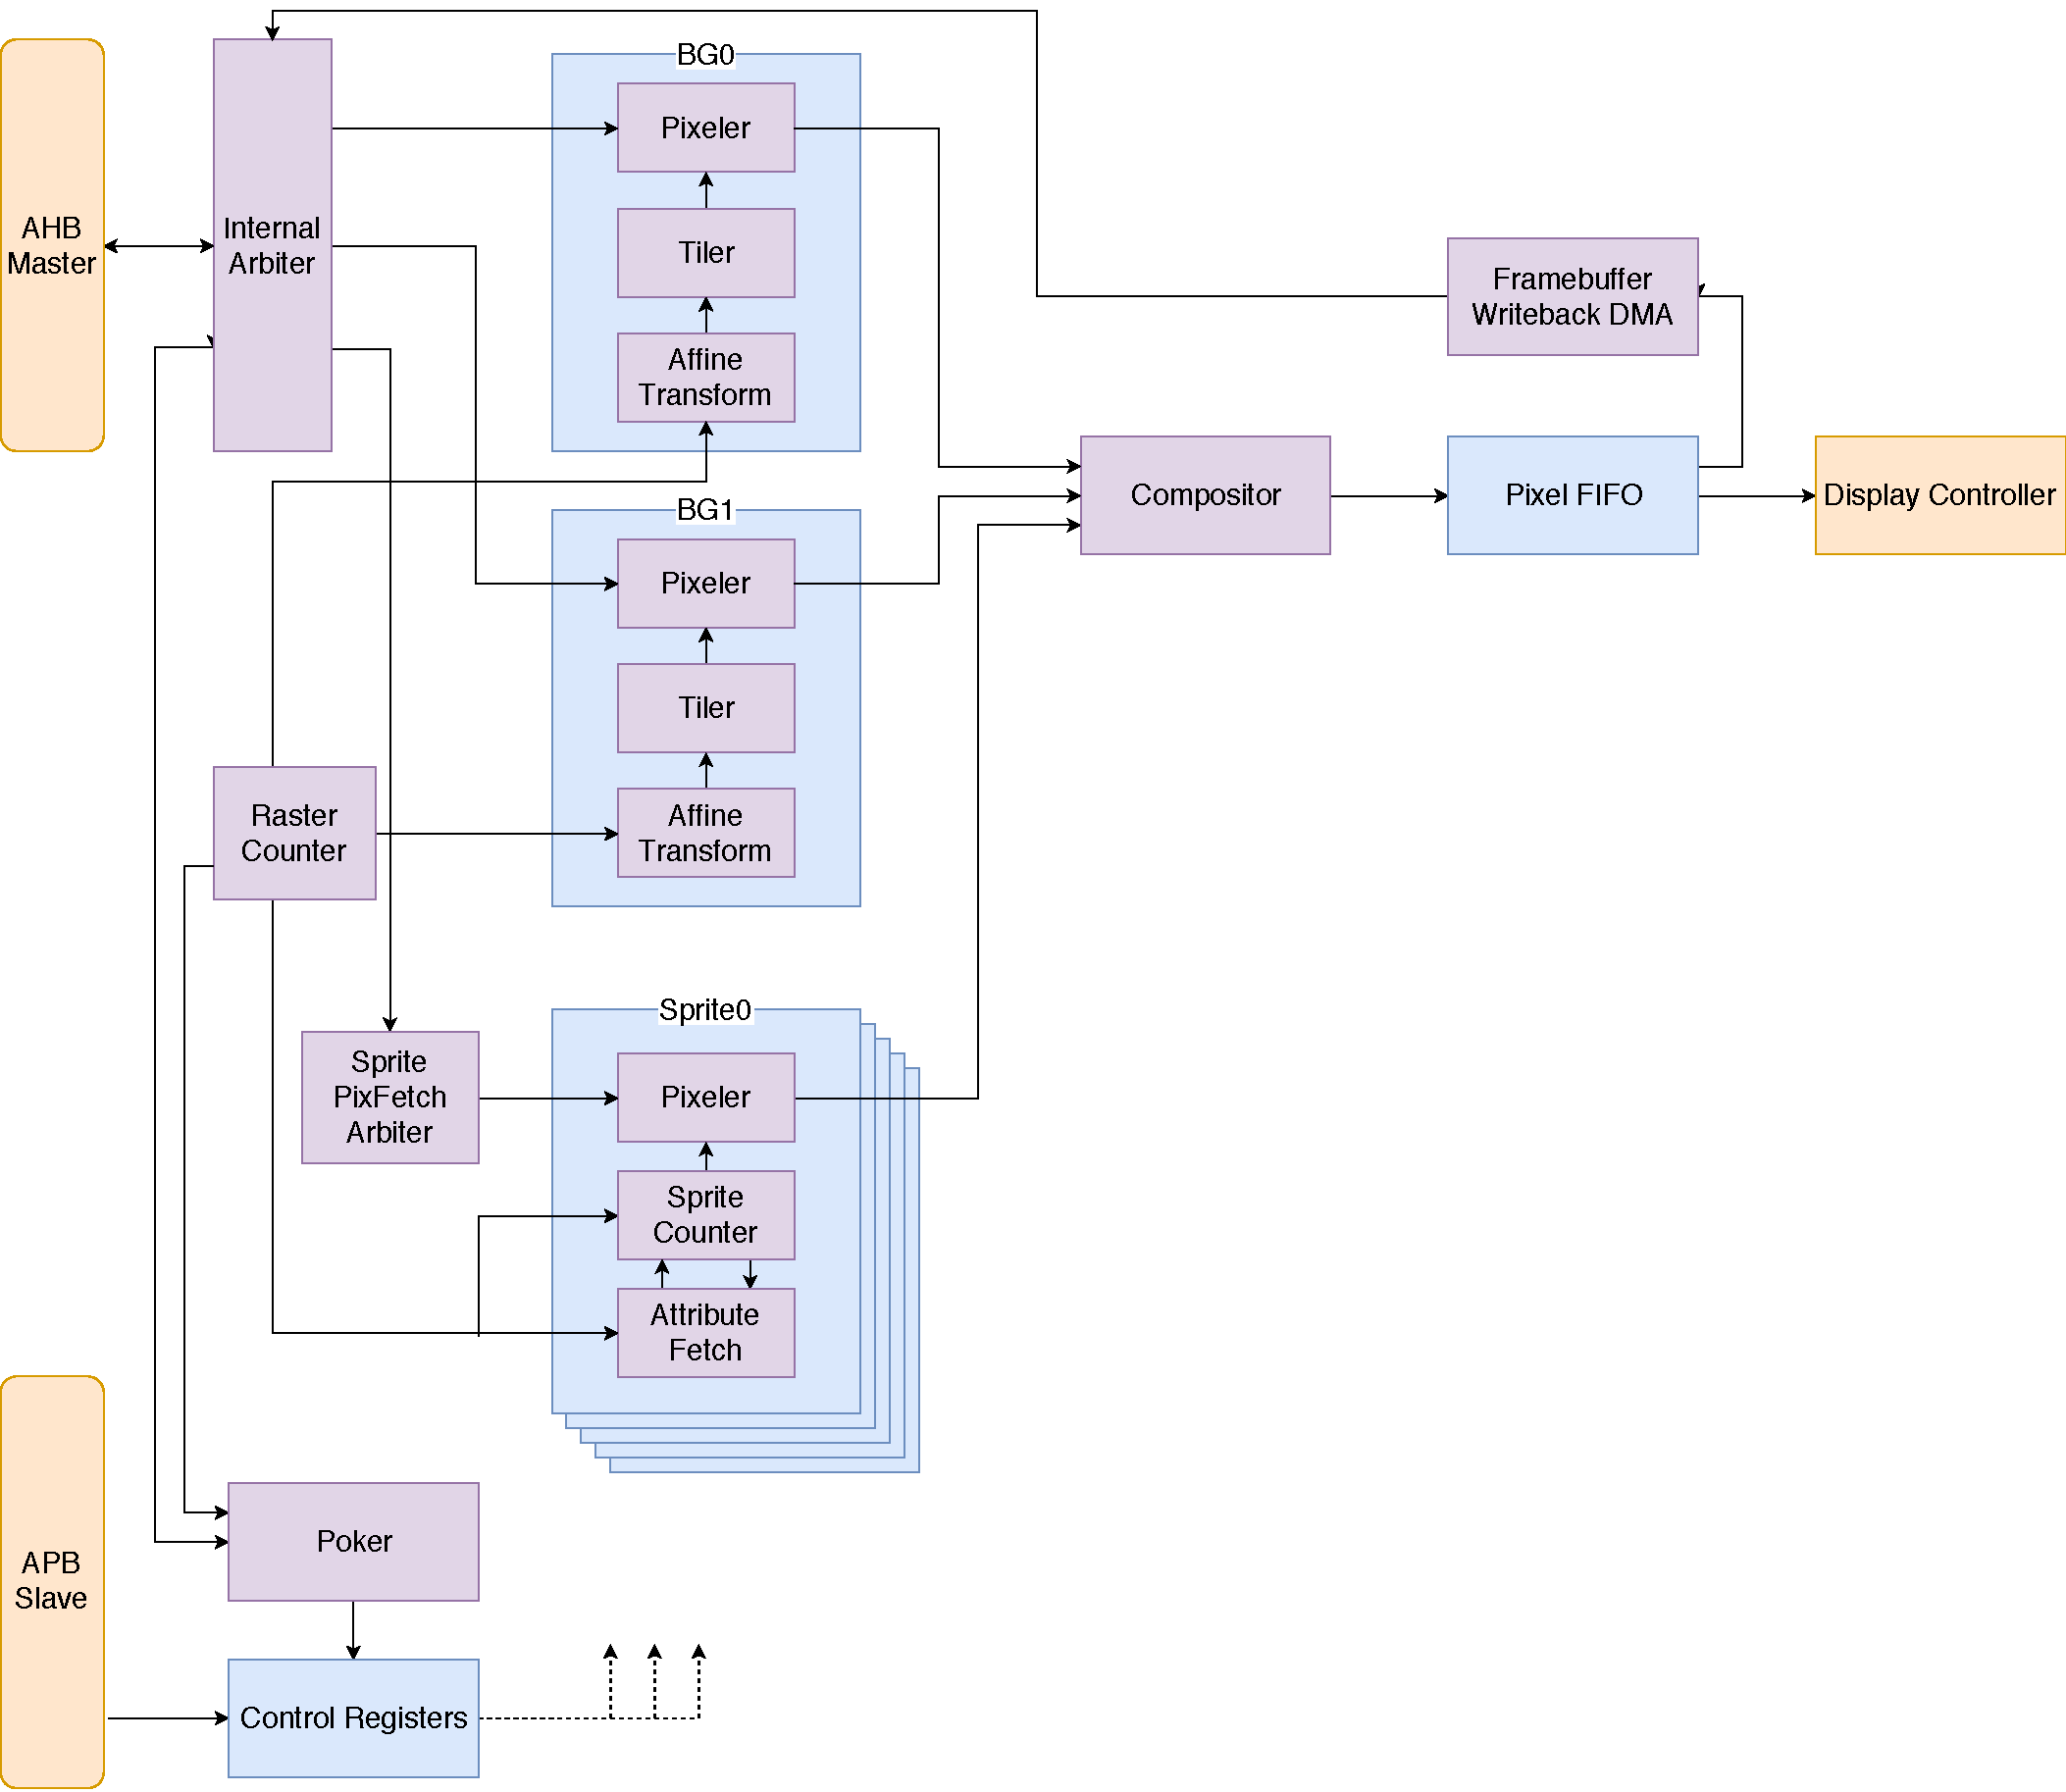
\includegraphics[width=0.9\textwidth]{diagrams/graphics.pdf}
\end{figure}

\section{Bus Fabric and Memory Subsystem}

AHB-lite single layer full crossbar, 32-bit datapath, no burst support. Low-bandwidth peripherals attached with an AHB-APB bridge + splitter. Written from scratch, so no guarantees that it works.

External 0.5MiB asynchronous SRAM with 16-bit data bus, 10 ns access times

\end{document}